%---------------------------------------------------------------------
\section{Expected Results}
\label{exp-performance}

In this section we present results regarding the expected performance
of the analysis. To obtain these results the number of observed events
has been set equal to the expected signal, according to the standard
model prediction, plus the expected background.

Figures.~\ref{exp-post-1d-2j} and \ref{exp-post-1d-3j} show the
resulting $tb$+$tqb$ posterior for the combined $e$+$\mu$ $\geq$~1
$b$-tag channel in two-jet and three-jet events.
Figure~\ref{exp-post-1d-allj} shows the $tb$+$tqb$ posterior for the
combination of all channels. The left figures correspond to the case
of only statistical uncertainties considered, whereas the right
figures also include systematic uncertainties.

\vspace{0.1in}
\begin{figure}[!h!tbp]
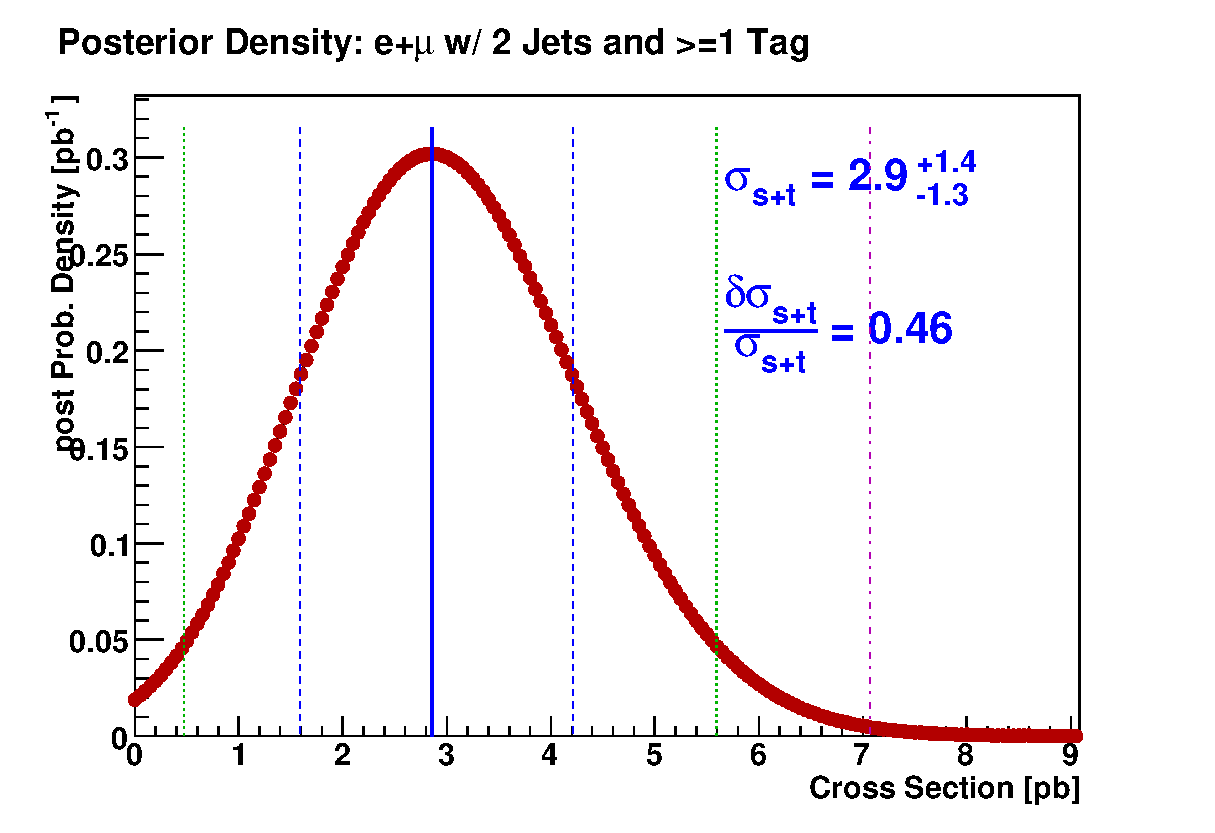
\includegraphics[width=0.37\textwidth]
{figures/posterior/nosys/expected_limit_TBTQ_LeptonsCombined_2Jet_TagsCombined}
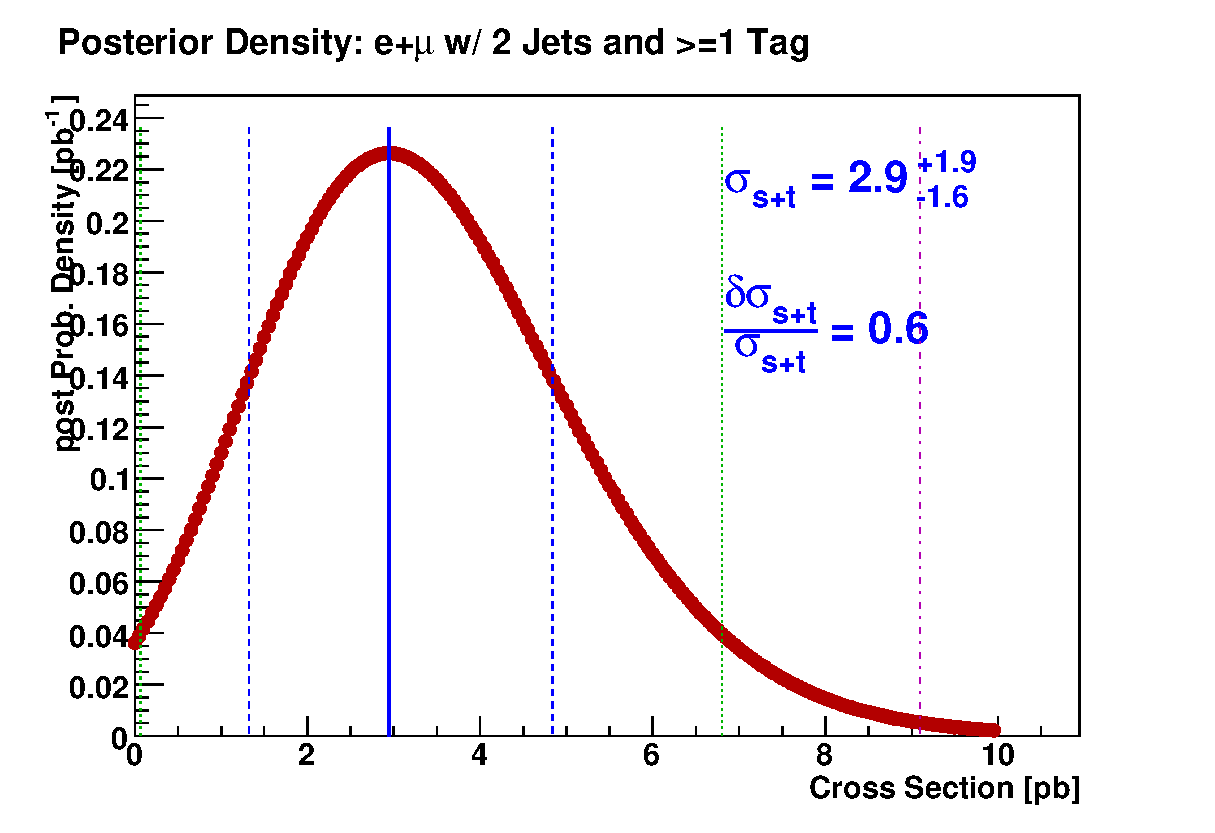
\includegraphics[width=0.37\textwidth]
{figures/posterior/sys/expected_limit_TBTQ_LeptonsCombined_2Jet_TagsCombined}
\vspace{-0.1in}
\caption[exppost1d2j]{Expected 1D posterior plots for the combined
$e$+$\mu$ $\geq$~1 $b$-tag channel in two-jet events, with statistical
uncertainties only (left plot) and including also systematic
uncertainties (right plot).}
\label{exp-post-1d-2j}
\end{figure}

\vspace{0.1in}
\begin{figure}[!h!tbp]
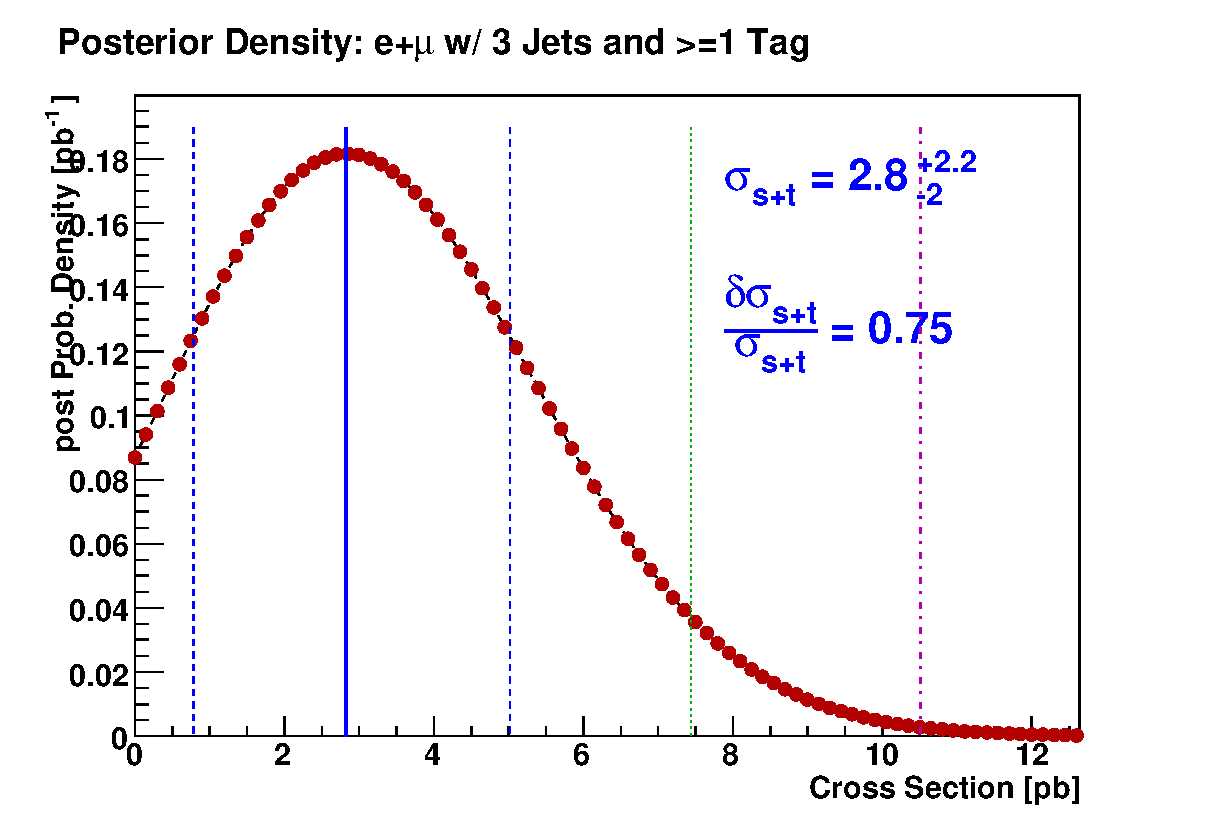
\includegraphics[width=0.37\textwidth]
{figures/posterior/nosys/expected_limit_TBTQ_LeptonsCombined_3Jet_TagsCombined}
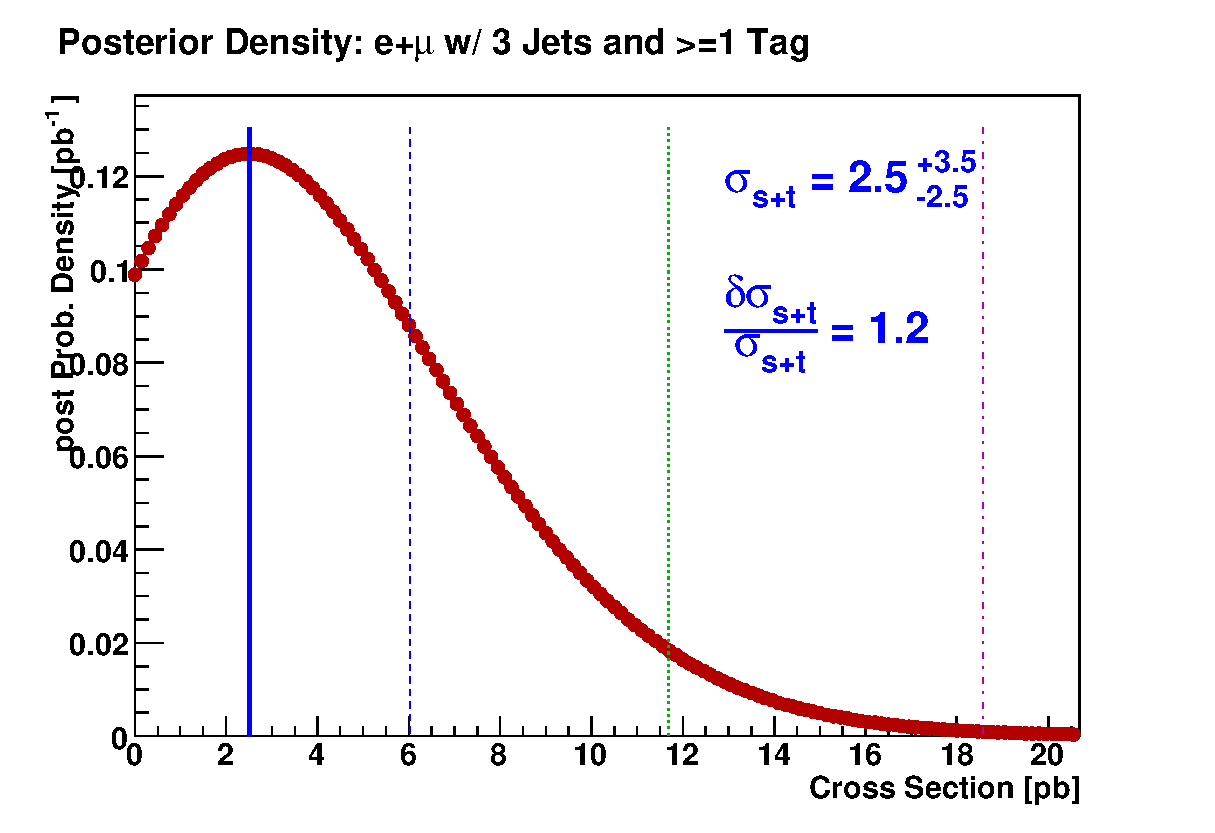
\includegraphics[width=0.37\textwidth]
{figures/posterior/sys/expected_limit_TBTQ_LeptonsCombined_3Jet_TagsCombined}
\vspace{-0.1in}
\caption[exppost1d3j]{Expected 1D posterior plots for the combined
$e$+$\mu$ $\geq$~1 $b$-tag channel in three-jet events, with
statistical uncertainties only (left plot) and including also
systematic uncertainties (right plot).}
\label{exp-post-1d-3j}
\end{figure}

\vspace{0.1in}
\begin{figure}[!h!tbp]
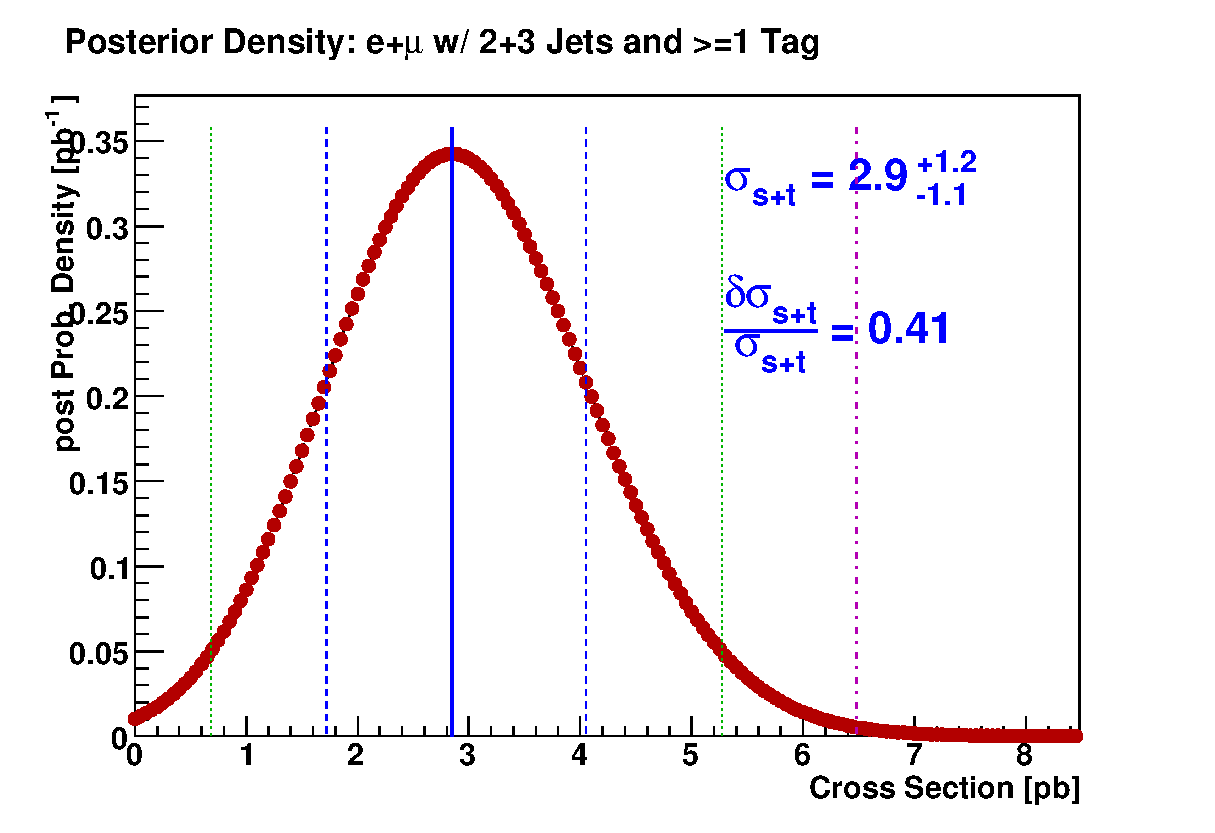
\includegraphics[width=0.37\textwidth]
{figures/posterior/nosys/expected_limit_TBTQ_LeptonsCombined_JetsCombined_TagsCombined}
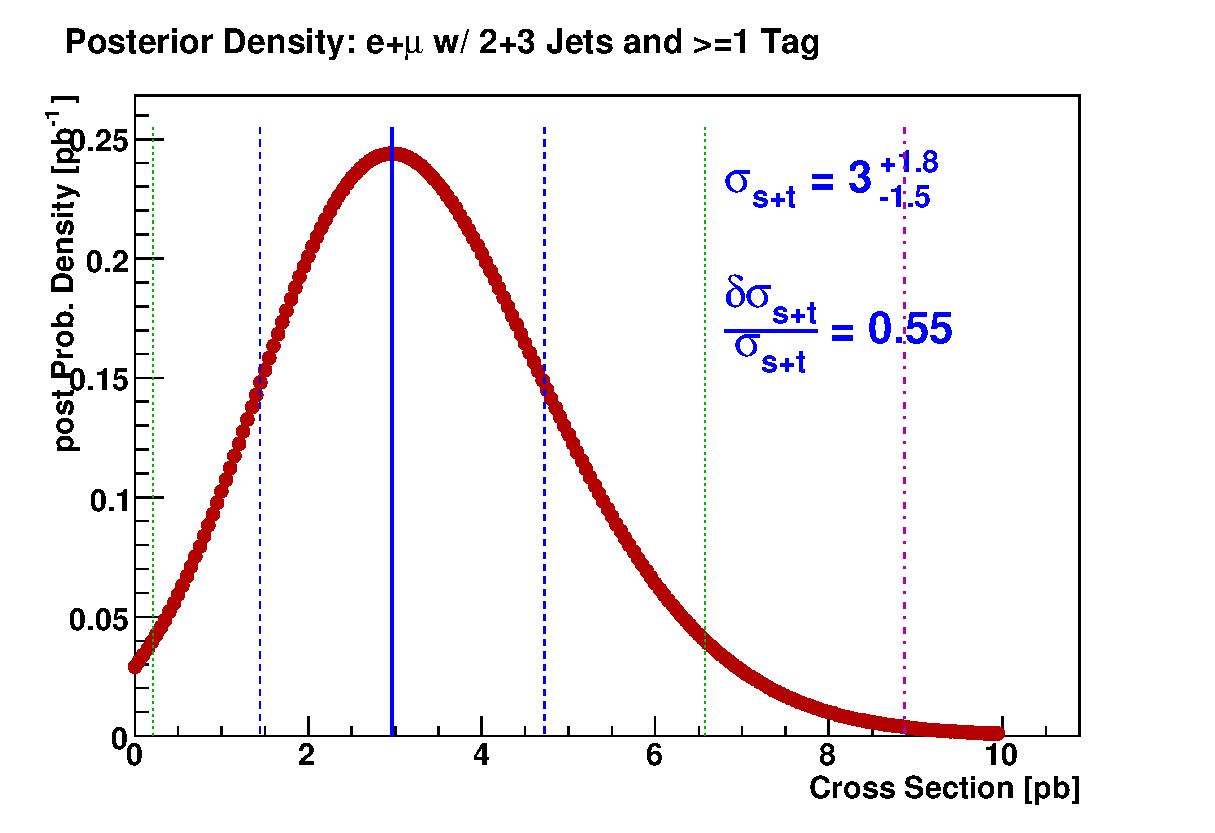
\includegraphics[width=0.37\textwidth]
{figures/posterior/sys/expected_limit_TBTQ_LeptonsCombined_JetsCombined_TagsCombined}
\vspace{-0.1in}
\caption[exppost1dallj]{Expected 1D posterior plots for the
combination of all channels, with statistical uncertainties only (left
plot) and including also systematic uncertainties (right plot).}
\label{exp-post-1d-allj}
\end{figure}

\subsection{Expected Signal Significance}

We calculate the significance of the expected results using the
$tb$+$tqb$ posteriors presented in the previous section. The Bayes
ratio (see Appendix~10 in Ref.~\cite{general-note}) is defined as the
peak value of the posterior divided by the posterior at zero signal
cross section. The larger the Bayes ratio, the larger the expected
significance of the result. This measure has been used to optimize the
analysis in the individual channels.  Results are shown in
Table~\ref{bayes-ratio}.

\begin{table}[!h!tbp]
\begin{center}
\begin{minipage}{5in}
\begin{ruledtabular}
\begin{tabular}{l|cc|cc|cc|c}
  \multicolumn{8}{c}{\hspace{0.5in}\underline{Expected Bayes Ratios for the $tb$+$tqb$ Signal}}\vspace{0.1in}\\
& \multicolumn{2}{c|}{1,2tags + 2,3jets}& \multicolumn{2}{c|}{$e$,$\mu$ + 2,3jets}
& \multicolumn{2}{c|}{$e$,$\mu$ + 1,2tags}& All \\
                 &  $e$-chan & $\mu$-chan& 1 tag & 2 tags& 2 jets& 3 jets&channels\\
\hline
Statistics only  &  $8.1$  & $4.1$ & $17.8$ & $1.9$ & $15.9$ & $2.1$ & $33.3$     \\
With systematics &  $3.8$  & $2.6$ & $6.3$  & $1.4$ & $6.2$  & $1.3$ & $\mathbf{8.4}$     \\
\end{tabular}
\end{ruledtabular}
\vspace{-0.1in}
\caption[bayesratio]{Expected Bayes ratios, without and with
systematic uncertainties, for many combinations of analysis
channels. The best value from all channels combined, with
systematics, is shown in bold type.}
\label{bayes-ratio}
\end{minipage}
\end{center}
\end{table}

% AJ 11/18/2006  
% I'm commenting this out since this S/sqrt{B} would best be evaluated
% cutting on the s+t discriminant
%
%A third method is to calculate the expected signal divided by the
%$\sqrt{B}$ for a particular cut on either the $s$-channel or
%$t$-channel discriminant. A grid search was performed on each analysis
%channel to determined the best $S/\sqrt{B}$. These values are
%summarized in Table~\ref{exp-srootb}.
%
%\begin{table}[!h!tbp]
%\begin{center}
%\begin{minipage}{3 in}
%\begin{ruledtabular}
%\begin{tabular}{l||ccc}
%\multicolumn{4}{c}
%{\hspace{0.1in}\underline{Best Expected $S/\sqrt{B}$ for the $tb$+$tq$ Signal}}\vspace{0.05in} \\
%                & $e$-chan & $\mu$-chan & Combined \\
%\hline
%With systematics&          &            &          \\
%~~Signal        &   12     &      9     &    21        \\
%~~Background    &   74     &     67     &   141        \\
%~~$S/\sqrt{B}$  &  1.4     &    1.1     &   1.8        
%\end{tabular}
%\end{ruledtabular}
%\vspace{-0.1 in}
%\caption[expsrootb]{Best expected significance on the total single
%top cross section for the 1-tag and 2-tags channels combined.}
%\label{exp-srootb}
%\end{minipage}
%\end{center}
%\end{table}
%
%\clearpage

\vspace{-0.1in}

\subsection{Expected Cross Section}

Table~\ref{tab:expxsecs} shows the expected cross sections for various
combinations of analysis channels. The expected result for each
combination is consistent with the standard model cross
section. Table~\ref{exp-errors} summarizes the relative uncertainty on
the expected $tb$+$tqb$ cross section measurement, defined as half the
width of the $tb$+$tqb$ posterior, divided by the cross section value
at the posterior peak.

\begin{table}[!h!tbp]
\begin{center}
\begin{minipage}{5in}
\begin{ruledtabular}
\begin{tabular}{l|cc|cc|cc|c}
  \multicolumn{8}{c}{\hspace{0.5in}\underline{Expected $tb$+$tqb$ Cross Section}}\vspace{0.1in}\\
& \multicolumn{2}{c|}{1,2tags + 2,3jets}& \multicolumn{2}{c|}{$e$,$\mu$ + 2,3jets}
& \multicolumn{2}{c|}{$e$,$\mu$ + 1,2tags}& All \\
                 &  $e$-chan & $\mu$-chan& 1 tag & 2 tags& 2 jets& 3 jets&channels\\
\hline
Statistics only  &  $2.8^{+1.5}_{-1.4}$  & $2.8^{+1.8}_{-1.7}$ & $2.9^{+1.3}_{-1.2}$ & $2.8^{+2.5}_{-2.2}$ & $2.9^{+1.4}_{-1.3}$ & $2.8^{+2.2}_{-2.1}$ & $2.9^{+1.2}_{-1.1}$ \\
With systematics &  $3.0^{+2.2}_{-1.8}$  & $3.1^{+2.5}_{-2.1}$ & $2.9^{+1.8}_{-1.6}$ & $2.7^{+3.4}_{-2.7}$ & $2.9^{+1.9}_{-1.6}$ & $2.5^{+3.5}_{-2.5}$ & $\mathbf{3.0^{+1.8}_{-1.5}}$ \\
\end{tabular}
\end{ruledtabular}
\vspace{-0.1in}
\caption[expxsecs]{Expected $tb$+$tqb$ cross sections, without and
with systematic uncertainties, for many combinations of the analysis
channels. The final expected result of this analysis are shown in the
lower right hand corner in bold type.}
\label{tab:expxsecs}
\end{minipage}
\end{center}
\end{table}

\vspace{-0.1in}
\begin{table}[!h!tbp]
\begin{center}
\begin{minipage}{5in}
\begin{ruledtabular}
\begin{tabular}{l|cc|cc|cc|c}
  \multicolumn{8}{c}{\hspace{0.5in}\underline{Relative Uncertainties on the Expected $tb$+$tqb$ Cross Section}}\vspace{0.1in}\\
& \multicolumn{2}{c|}{1,2tags + 2,3jets}& \multicolumn{2}{c|}{$e$,$\mu$ + 2,3jets}
& \multicolumn{2}{c|}{$e$,$\mu$ + 1,2tags}& All \\
                 &  $e$-chan & $\mu$-chan& 1 tag & 2 tags& 2 jets& 3 jets&channels\\
\hline
Statistics only  &  $52\%$  & $60\%$ & $45\%$ & $83\%$  &  $46\%$  & $75\%$  & $41\%$     \\
With systematics &  $67\%$  & $75\%$ & $59\%$ & $115\%$ &  $60\%$  & $121\%$ & $\mathbf{55\%}$     \\
\end{tabular}
\end{ruledtabular}
\vspace{-0.1in}
\caption[exp-errors]{Relative uncertainties on the expected
$tb$+$tqb$ cross section, without and with systematic uncertainties,
for many combinations of the analysis channels. The best value from
all channels combined, with systematics, is shown in bold type.}
\label{exp-errors}
\end{minipage}
\end{center}
\end{table}

%Figs.~\ref{exp-post-1d} and \ref{exp-post-2d} show the 1D posterior
%and 2D posteriors for the case of expected standard model signal.

%\vspace{0.1in}
%\begin{figure}[!h!tbp]
%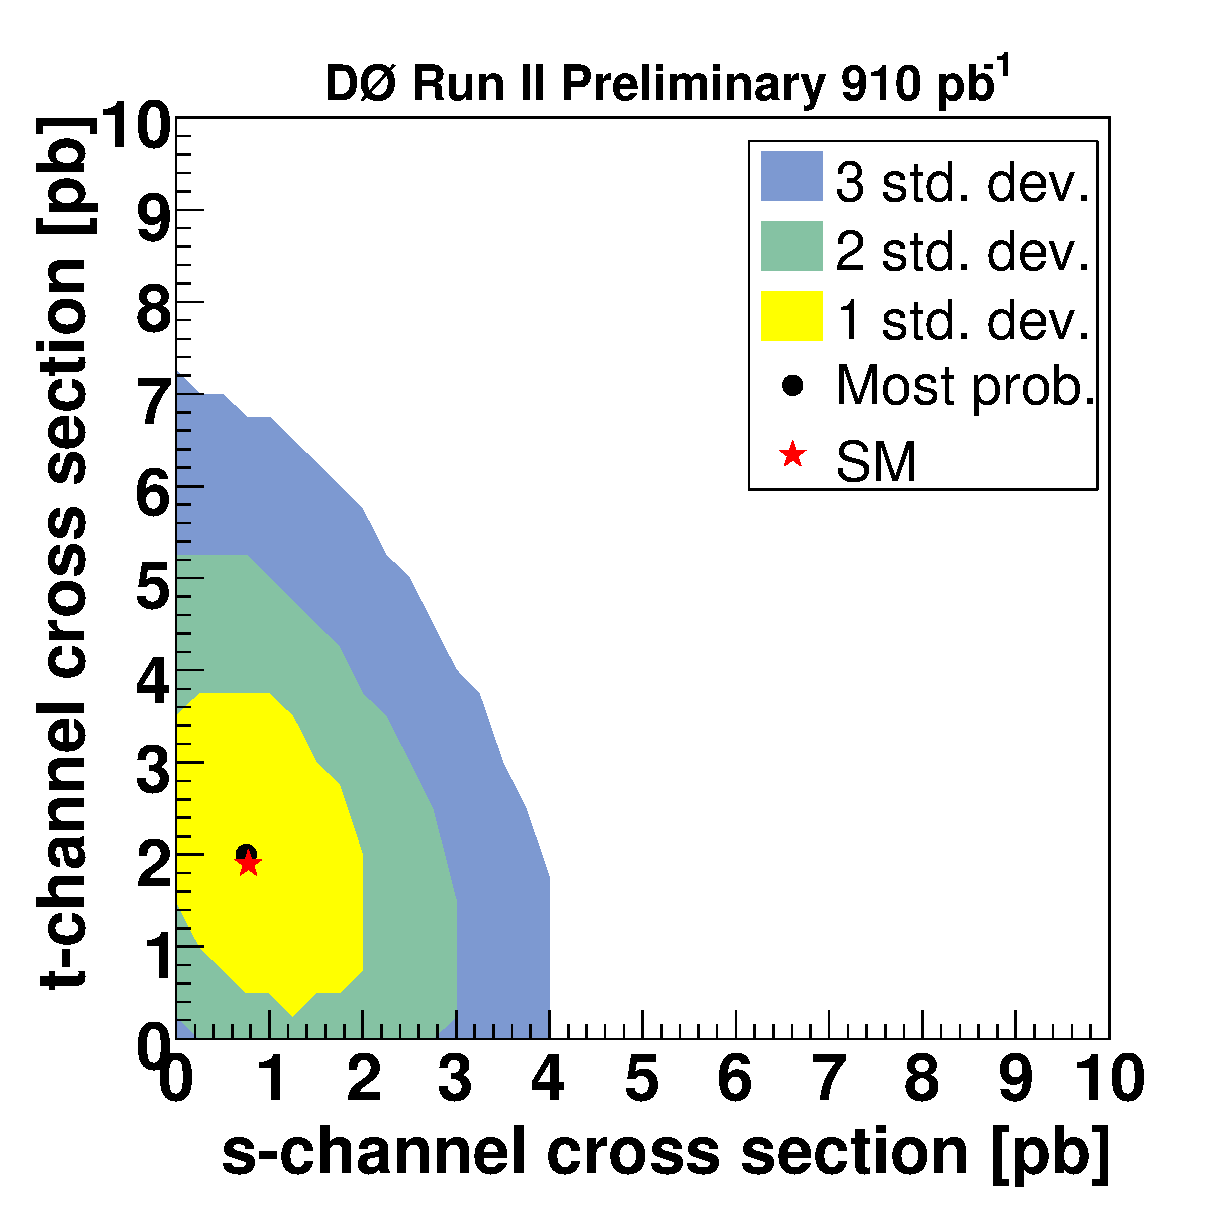
\includegraphics[width=0.37\textwidth]{figures/posterior/nosys/2D-Posterior_LeptonsCombined_2Jet_TagsCombined_expected_limit.eps}
%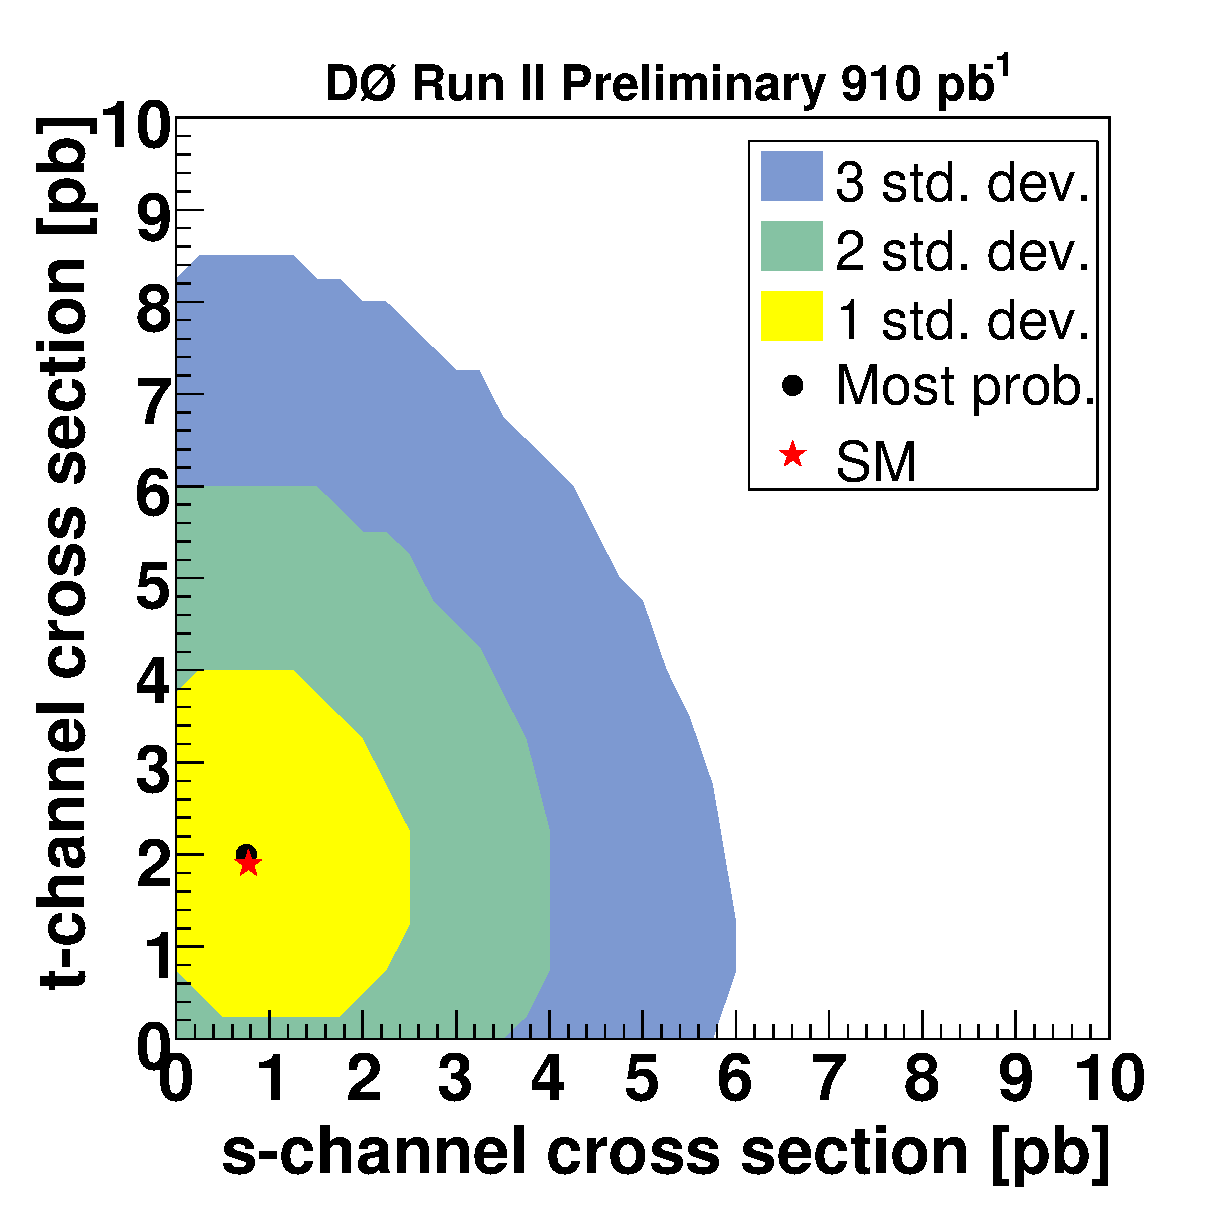
\includegraphics[width=0.37\textwidth]{figures/posterior/sys/2D-Posterior_LeptonsCombined_2Jet_TagsCombined_expected_limit.eps}
%\vspace{-0.1in}
%\caption[exppost2d]{Expected 2D posterior plots for the combined
%$e$+$\mu$ $\geq$~1 $b$-tag channel with statistical uncertainties only
%(left plot) and with systematic uncertainties as well (right plot).}
%\label{exp-post-2d}
%\end{figure}
